\documentclass[11pt,letterpaper]{article}
\usepackage[margin=0.88in]{geometry}
\usepackage[T1]{fontenc}
\usepackage[utf8]{inputenc}
\usepackage{lmodern,amsmath,amssymb,mathtools,amsthm,microtype}
\usepackage{tikz}
\usetikzlibrary{arrows.meta,angles,quotes,calc,positioning}
\usepackage{xcolor,enumitem,array,booktabs,hyperref}
\hypersetup{colorlinks=true,linkcolor=blue!45!black,urlcolor=blue!45!black}
\definecolor{deepblue}{RGB}{27,70,120}
\definecolor{tealblue}{RGB}{0,118,118}
\definecolor{warmorange}{RGB}{170,96,25}
\definecolor{softblue}{RGB}{234,243,250}
\definecolor{softgray}{RGB}{247,248,249}
% Semantic marker strokes. Input after preamble.tex; no package options added.
\ifdefined\GTenHighlightLoaded\endinput\fi
\let\GTenHighlightLoaded\relax
\RequirePackage{tikz} % Already loaded by the shared preamble; loaded only once.
\definecolor{GTenHLValue}{HTML}{FFBB55}
\definecolor{GTenHLSecond}{HTML}{8FD49A}
\definecolor{GTenHLThird}{HTML}{F1DA55}
\definecolor{GTenHLOutcome}{HTML}{BC9DE0}
\definecolor{GTenHLProbability}{HTML}{86BFF0}
\definecolor{GTenHLParameter}{HTML}{ED9DAA}
\newif\ifGTenHighlights
\GTenHighlightstrue
% Switch off with \GTenHighlightsfalse (restore with \GTenHighlightstrue).
% Every role command accepts ONE short text OR math fragment, in its current
% mode: \GTenHLValue{buyers}, $\GTenHLValue{X}_i^2$,
% \[p_X(\GTenHLValue{1})=\GTenHLProbability{0.5}.\]
% In aligned equations keep &, \\, relation signs and binary operators OUTSIDE
% strokes; highlight atoms/short phrases, not whole calculations. Do not nest
% strokes. For text within math use \text, e.g. \GTenHLOutcome{\text{cash}}.
% mathpalette preserves display/text/script/scriptscript sizes without nesting
% an equation environment. The node's base is exactly the content's baseline.
% Only the background is translucent; glyphs retain their current color.
\tikzset{gten marker/.style={rectangle,rounded corners=1mm,draw=none,fill=#1,
  fill opacity=.32,text opacity=1,inner xsep=1.5mm,inner ysep=0.8mm,
  outer sep=0pt}}
% Private implementation avoids LaTeX @ names so this input needs no catcode
% changes. \mathsurround is reset locally inside each math node.
\newcommand{\GTenHLMathStroke}[2]{%
  \tikz[baseline=(gtenhl.base)]\node[gten marker=\GTenHLCurrentColor]
    (gtenhl) {$\mathsurround=0pt #1#2$};}
\newcommand{\GTenHLStroke}[2]{%
  \ifGTenHighlights
    \begingroup\def\GTenHLCurrentColor{#1}%
    \ifmmode\mathpalette\GTenHLMathStroke{#2}%
    \else\tikz[baseline=(gtenhl.base)]\node[gten marker=#1]
      (gtenhl) {#2};\fi
    \endgroup
  \else#2\fi}
% Roles: Value = primary variable and its values/units; Second/Third = other
% simultaneous variables; Outcome = complete outcome or label; Probability =
% known masses/results; Parameter = mass/constant being determined, including
% its solved value (which uses Probability when substituted as a known mass).
\newcommand{\GTenHLValue}[1]{\GTenHLStroke{GTenHLValue}{#1}}
\newcommand{\GTenHLSecond}[1]{\GTenHLStroke{GTenHLSecond}{#1}}
\newcommand{\GTenHLThird}[1]{\GTenHLStroke{GTenHLThird}{#1}}
\newcommand{\GTenHLOutcome}[1]{\GTenHLStroke{GTenHLOutcome}{#1}}
\newcommand{\GTenHLProbability}[1]{\GTenHLStroke{GTenHLProbability}{#1}}
\newcommand{\GTenHLParameter}[1]{\GTenHLStroke{GTenHLParameter}{#1}}
% Legends stay readable in monochrome: names and units carry the meaning.
\newcommand{\GTenHighlightLegend}{%
  \textbf{Marker key:} \GTenHLValue{variable and values};
  \GTenHLOutcome{outcomes}; \GTenHLProbability{probabilities};
  \GTenHLParameter{parameter to determine}.
  When variables occur together: \GTenHLValue{$X$ (buyers)},
  \GTenHLSecond{$Y$ (USD)}, \GTenHLThird{$Z$ (indicator)}.
  Match each value to its variable's marker; probability markers have no units.}

% \GTenHighlightsfalse % Uncomment to disable instructional highlights.
\newcommand{\vect}[1]{\boldsymbol{#1}}
\newcommand{\R}{\mathbb{R}}
\newcommand{\norm}[1]{\left\lVert #1\right\rVert}
\newcommand{\abs}[1]{\left\lvert #1\right\rvert}
\newcommand{\role}[2]{\ifGTenHighlights\textcolor{#1}{#2}\else#2\fi}
\newcommand{\along}[1]{\role{warmorange}{#1}}
\newcommand{\height}[1]{\role{tealblue}{#1}}
\newcommand{\keyeq}[1]{\begin{center}\fbox{\parbox{.91\linewidth}{\centering$\displaystyle #1$}}\end{center}}
\newcommand{\tagword}[1]{\textbf{#1.}}
\setlength{\parindent}{0pt}
\setlength{\parskip}{.5em}
\setlist[enumerate]{itemsep=.32em,topsep=.3em}
\raggedbottom
% Unbreakable top-aligned pairs: explanations and diagrams never become floats.
\newcounter{teachingstep}[section]
\newcommand{\teach}[3]{\par\addvspace{1em}\noindent
\begin{minipage}{\linewidth}
\refstepcounter{teachingstep}\textbf{Step \arabic{teachingstep}. #1}\par\smallskip
\begin{minipage}[t]{.575\linewidth}\vspace{0pt}#2\end{minipage}\hfill
\begin{minipage}[t]{.39\linewidth}\vspace{0pt}\centering#3\end{minipage}
\end{minipage}\par}
\newcommand{\pausepredict}[2]{\par\smallskip\textbf{Pause and predict.} #1\par\textit{Explanation.} #2}
\tikzset{>=Stealth,
 uvec/.style={->,very thick,draw=\ifGTenHighlights deepblue\else black\fi},
 vvec/.style={->,thick,densely dashed,draw=\ifGTenHighlights tealblue\else black\fi},
 focus/.style={very thick,draw=\ifGTenHighlights warmorange\else black\fi},
 high/.style={thick,densely dashed,draw=\ifGTenHighlights tealblue\else black\fi},
 faint/.style={thin,draw=gray!55},
 panel/.style={font=\small,line cap=round,line join=round},
 shade/.style={fill=\ifGTenHighlights softblue\else none\fi}}
% Fixed acute sequence: OB=4, H=(1.5,0), C=(1.5,2.2).
% Modes: 0 vectors; 1 perpendicular; 2 projection; 3 height; 4 BHC; 5 OHC.
\newcommand{\trianglepanel}[1]{%
\begin{tikzpicture}[panel,scale=.91]
\coordinate (O) at (0,0);\coordinate (B) at (4,0);
\coordinate (C) at (1.5,2.2);\coordinate (H) at (1.5,0);
\ifnum#1=4 \path[shade] (B)--(H)--(C)--cycle;\fi
\ifnum#1=5 \path[shade] (O)--(H)--(C)--cycle;\fi
\draw[faint] (-.2,0)--(4.2,0);
\draw[uvec] (O)--(B) node[pos=.8,below=15pt] {$\vect u,\ p$};
\draw[vvec] (O)--(C) node[midway,above left] {$\vect v,\ q$};
\ifnum#1>0\ifnum#1=6\else
\draw[high] (C)--(H);\draw[faint] (1.5,.17)--(1.67,.17)--(1.67,0);
\node[below right] at (H) {$H$};\fi\fi
\ifnum#1=2 \draw[focus,->] (O)--(H);\node[below=19pt] at (.5,0) {$x=q\cos\theta$};\fi
\ifnum#1=3 \draw[focus] (H)--(C) node[midway,right] {$h=q\sin\theta$};\fi
\ifnum#1>3
\ifnum#1=5 \draw[faint] (C)--(B) node[midway,above right] {$s$};
\draw[focus,densely dashed] (O)--(C);
\draw[focus] (O)--(H);\draw[focus,densely dashed] (H)--(C);
\else
\ifnum#1=7 \draw[faint] (C)--(B) node[midway,above right] {$s$};
\draw[focus,<->] (H)--(B);
\else \draw[focus,->] (C)--(B) node[midway,above right] {$s$};\fi\fi
\ifnum#1=6\else
\node[right] at (1.5,1.1) {$h$};\node[below] at (.65,0) {$x$};
\node[below] at (2.85,0) {$|p-x|$};\fi
\ifnum#1=4 \draw[focus] (H)--(B);\draw[focus,densely dashed] (H)--(C);\fi
\fi
\pic[draw,angle radius=.48cm,angle eccentricity=1.5,"$\theta$"] {angle=B--O--C};
\node[below left] at (O) {$O$};\node[below right] at (B) {$B$};\node[above] at (C) {$C$};
\end{tikzpicture}}
\newcommand{\casepanel}[3]{%
\begin{tikzpicture}[panel,scale=.78]
\coordinate (O) at (0,0);\coordinate (B) at (3,0);
\coordinate (C) at (#1,#2);\coordinate (H) at (#1,0);
\draw[faint] (-1.7,0)--(4.3,0);\draw[uvec] (O)--(B);\draw[vvec] (O)--(C);
\draw[focus] (C)--(B) node[midway,above right] {$s$};
\draw[high] (C)--(H) node[midway,right] {$h$};
\draw[faint] (#1,.15)--++(.15,0)--++(0,-.15);
\ifdim#1pt=0pt \node[below left] at (O) {$O=H$};
\else \node[below] at (O) {$O$};\node[below left] at (H) {$H$};\fi
\node[below] at (B) {$B$};\node[above] at (C) {$C$};
\node[align=center] at (1.1,-.85) {#3};
\end{tikzpicture}}
\newcommand{\parapanel}[1]{%
\begin{tikzpicture}[panel,scale=.84]
\coordinate (O) at (0,0);\coordinate (B) at (4,0);\coordinate (C) at (1.5,2.2);\coordinate (W) at (5.5,2.2);
\ifnum#1>0 \path[shade] (O)--(B)--(W)--(C)--cycle;
\draw[faint] (B)--(W)--(C);\node[above] at (W) {$W:\ \vect u+\vect v$};\fi
\draw[uvec] (O)--(B) node[pos=.8,below=15pt] {$p,\ \vect u$};
\draw[vvec] (O)--(C) node[midway,left] {$q,\ \vect v$};
\ifnum#1=1 \draw[focus,->] (O)--(W);\fi
\ifnum#1>1 \draw[high] (C)--(1.5,0) node[midway,right] {$h$};
\draw[faint] (1.5,.17)--(1.67,.17)--(1.67,0);\node[below] at (1.5,0) {$H$};\fi
\node[below left] at (O) {$O$};\node[below right] at (B) {$B$};\node[above] at (C) {$C$};
\end{tikzpicture}}
% Actual Example 1 coordinates with equal axis scales, unchanged between panels.
\newcommand{\examplepanel}[1]{%
\begin{tikzpicture}[panel,scale=.70]
\coordinate (O) at (0,0);\coordinate (B) at (3,1);\coordinate (C) at (2,4);\coordinate (W) at (5,5);
\draw[faint,->] (-.4,0)--(5.5,0) node[right] {$x$};
\draw[faint,->] (0,-.4)--(0,5.6) node[above] {$y$};
\foreach \x in {1,...,5}{\draw[faint] (\x,.06)--(\x,-.06) node[below,font=\scriptsize] {\x};}
\foreach \y in {1,...,5}{\draw[faint] (.06,\y)--(-.06,\y) node[left,font=\scriptsize] {\y};}
\ifnum#1>1 \path[shade] (O)--(B)--(W)--(C)--cycle;\draw[faint] (B)--(W)--(C);\node[above] at (W) {$(5,5)$};\fi
\draw[uvec] (O)--(B) node[right] {$B(3,1)$};
\draw[vvec] (O)--(C) node[above left] {$C(2,4)$};
\ifnum#1>0 \draw[high] (C)--(B) node[midway,right] {$h=\sqrt{10}$};
\draw[faint] ($(B)+(-.18,-.06)$)--++(-.06,.18)--++(.18,.06);
\pic[draw,angle radius=.7cm,angle eccentricity=1.5,"$45^\circ$"] {angle=B--O--C};\fi
\ifnum#1=3 \draw[focus,->] (.75,.25) arc[start angle=18.435,end angle=63.435,radius=.79];\node at (3.5,3.2) {$D=+10$};\fi
\node[below left] at (O) {$O$};
\end{tikzpicture}}
\title{\vspace{-1.4em}\textbf{From the Dot Product to Oriented Area}\\[.3em]\large A Geometric Introduction to Determinants and the Wedge Product}
\author{}\date{}
\begin{document}
\maketitle\vspace{-1.5em}
\textbf{Learning goals.} Derive the law of cosines using projections and Pythagoras; prove the coordinate dot product; find parallelogram area; justify the determinant's orientation sign; and expand the wedge product with all four terms visible.

\textbf{Logical route.} Vectors $\to$ projections $\to$ Pythagoras $\to$ law of cosines $\to$ dot product $\to$ area $\to$ determinant $\to$ orientation $\to$ wedge product.

\textbf{Visual legend.} A solid arrow marks $\vect u$ (blue); a dashed arrow marks $\vect v$ (teal). Orange emphasizes a directed projection or the current comparison. A dashed perpendicular marks height. Faint lines retain earlier construction. Names and formulas keep their meaning in grayscale. Coordinate drawings have equal axis scales; term maps are explicitly algebraic schematics.

\section{Vectors, lengths, and angles}
Work in the Euclidean plane $\R^2$ with its standard orthonormal axes:
\[
\vect e_1=(1,0),\quad\vect e_2=(0,1),\qquad
\vect u=(a,b)=a\vect e_1+b\vect e_2,\quad\vect v=(c,d)=c\vect e_1+d\vect e_2.
\]
\teach{Read coordinates as displacements}{Start at $O$. Move horizontally by $a$, then vertically by $b$. The endpoint is $B=(a,b)$, so the direct arrow $OB$ is $\vect u$.

The pictured $a,b$ are positive. A negative coordinate means displacement in the opposite axis direction, not a negative physical length.}{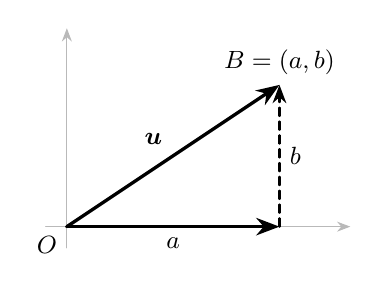
\begin{tikzpicture}[panel,scale=.9]
\draw[faint,->] (-.3,0)--(4,0);\draw[faint,->] (0,-.3)--(0,2.8);
\draw[focus,->] (0,0)--(3,0) node[midway,below] {$a$};
\draw[high,->] (3,0)--(3,2) node[midway,right] {$b$};
\draw[uvec] (0,0)--(3,2) node[midway,above left] {$\vect u$};
\node[above] at (3,2) {$B=(a,b)$};\node[below left] at (0,0) {$O$};
\end{tikzpicture}}
\newpage
\subsection*{Subtraction connects endpoints}
\teach{Draw both arrows from a common origin}{Use $\vect u=(3,1)$ and $\vect v=(1,2)$. Start both arrows at $O$ and name their tips $B$ and $C$.

Before subtracting, notice that the two tips are different. We will find the displacement that takes $C$ to $B$.}{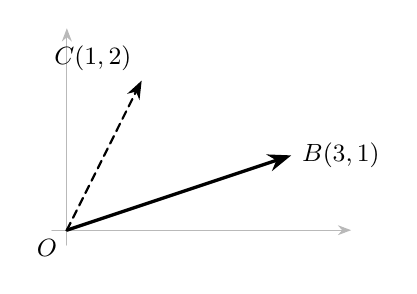
\begin{tikzpicture}[panel,scale=.95]
\draw[faint,->] (-.2,0)--(3.8,0);\draw[faint,->] (0,-.2)--(0,2.7);
\draw[uvec] (0,0)--(3,1) node[right] {$B(3,1)$};
\draw[vvec] (0,0)--(1,2) node[above left] {$C(1,2)$};
\node[below left] at (0,0) {$O$};\end{tikzpicture}}
\teach{Try a numerical displacement first}{Draw $\vect u=(3,1)$ and $\vect v=(1,2)$ from $O$. To go from $C=(1,2)$ to $B=(3,1)$, move $2$ units right and $1$ down:
\[
\overrightarrow{CB}=(2,-1)=(3-1,1-2).
\]
This endpoint displacement is $\vect u-\vect v$.}{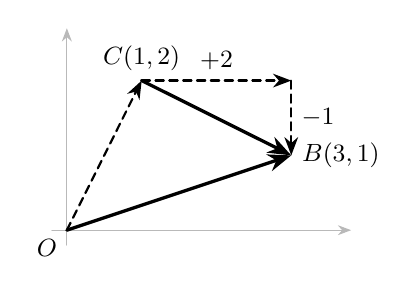
\begin{tikzpicture}[panel,scale=.95]
\draw[faint,->] (-.2,0)--(3.8,0);\draw[faint,->] (0,-.2)--(0,2.7);
\draw[uvec] (0,0)--(3,1) node[right] {$B(3,1)$};
\draw[vvec] (0,0)--(1,2) node[above] {$C(1,2)$};
\draw[focus,->] (1,2)--(3,1);
\draw[high,->] (1,2)--(3,2) node[midway,above] {$+2$};
\draw[high,->] (3,2)--(3,1) node[midway,right] {$-1$};
\node[below left] at (0,0) {$O$};\end{tikzpicture}}
\teach{Connect the general endpoints}{Keep the common tail $O$. Name the tips $B=(a,b)$ and $C=(c,d)$. Following the route $C\to O\to B$ gives
\[
\overrightarrow{CB}=-\vect v+\vect u=\vect u-\vect v.
\]
Equivalently, $\vect v+\overrightarrow{CB}=\vect u$. The dashed displacement route ends at the same $B$.}{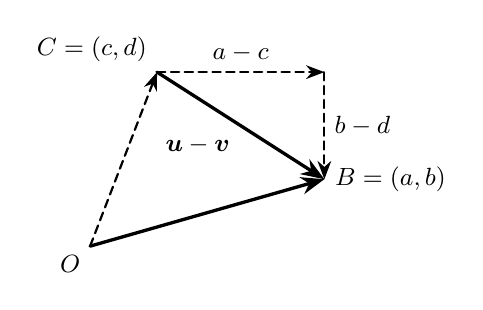
\begin{tikzpicture}[panel,scale=.85]
\draw[uvec] (0,0)--(3.5,1) node[right] {$B=(a,b)$};
\draw[vvec] (0,0)--(1,2.6) node[above left] {$C=(c,d)$};
\draw[focus,->] (1,2.6)--(3.5,1) node[midway,below left] {$\vect u-\vect v$};
\draw[high,->] (1,2.6)--(3.5,2.6) node[midway,above] {$a-c$};
\draw[high,->] (3.5,2.6)--(3.5,1) node[midway,right] {$b-d$};
\node[below left] at (0,0) {$O$};\end{tikzpicture}}
\tagword{Lengths from Pythagoras} Signed displacements become nonnegative squared lengths:
\[
\vect u-\vect v=(a-c,b-d),\qquad
\norm{\vect u}=\sqrt{a^2+b^2},\quad \norm{\vect v}=\sqrt{c^2+d^2},
\]
\[
\norm{\vect u-\vect v}^2=(a-c)^2+(b-d)^2.
\]
For nonzero vectors, $\theta\in[0,\pi]$ is their \emph{unoriented} included angle. A zero vector has no uniquely defined angle with another vector.


\newpage
\section{Projections and elementary trigonometry}
Assume both vectors are nonzero. Write $p=\norm{\vect u}$ and $q=\norm{\vect v}$. Rotate the \emph{drawing} so $OB$ points right; reflect the view if necessary so $C$ is above the line for this unoriented calculation. This preserves lengths and $\theta$. It does not assert that the original coordinates $(a,b)$ have become $(p,0)$. We will return to the original coordinate axes later.
\teach{Draw the two vectors}{Name the common tail $O$, the tip of $\vect u$ by $B$, and the tip of $\vect v$ by $C$. The angle $\theta=\angle BOC$ lies between sides of lengths $p$ and $q$.

First identify these sides. No dot product is being used.}{\trianglepanel{0}}
\teach{Drop a perpendicular to the whole line}{Let $H$ be the foot of the perpendicular from $C$ to the line $OB$. The right-angle mark says $CH\perp OB$.

Use the whole line, because $H$ need not lie between $O$ and $B$. This construction creates the right triangle needed for trigonometry.}{\trianglepanel{1}}
\teach{Name the signed shadow}{Let $x$ be the directed coordinate of $H$, measured from $O$ toward $B$:
\[
\along{x=q\cos\theta}.
\]
In the pictured acute triangle, $\cos\theta=OH/q$, so $x=OH>0$. This scalar is the signed component $\operatorname{comp}_{\vect u}(\vect v)$.}{\trianglepanel{2}}
\newpage
\subsection*{A height is a distance; a projection may be signed}
\teach{Name the nonnegative height}{The physical distance $CH=h$ is perpendicular to the base. In the pictured acute triangle, $\sin\theta=h/q$, hence
\[
\height{h=q\sin\theta}\ge0.
\]
For $\theta\in[0,\pi]$, sine remains nonnegative. The sloping side has length $q$; it is not the height.}{\trianglepanel{3}}
\teach{Compare the three angle types}{The foot $H$ can move across $O$. These panels use the same $p=3$, $q=\sqrt5$ and equal scales.

Acute: $x=1$, $h=2$.

Right: $x=0$, $h=\sqrt5$.

Obtuse: $x=-1$, $h=2$.

For the obtuse case, the acute reference angle is $\pi-\theta$. Thus
\[
OH=q\cos(\pi-\theta)=-q\cos\theta=|x|.
\]
The signed $x$ is negative while the length $OH$ is positive.}{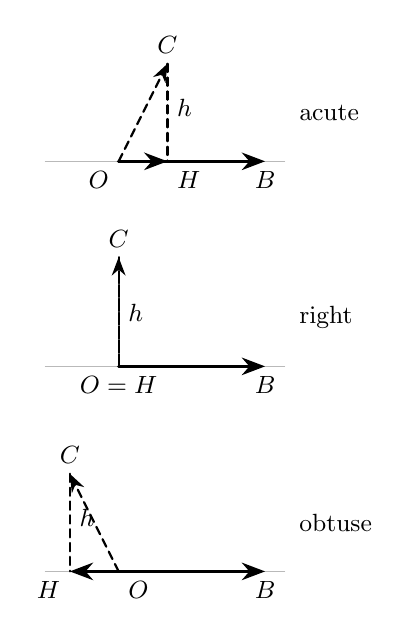
\begin{tikzpicture}[panel,scale=.62]
\foreach \xx/\yy/\lab/\shift in {1/2/acute/0,0/2.236/right/-4.2,-1/2/obtuse/-8.4}{
\begin{scope}[yshift=\shift cm]
\draw[faint] (-1.5,0)--(3.4,0);\draw[uvec] (0,0)--(3,0);
\draw[vvec] (0,0)--(\xx,\yy);\draw[high] (\xx,\yy)--(\xx,0);
\ifdim\xx pt=0pt \node[below] at (0,0) {$O=H$};
\else
\ifdim\xx pt>0pt \node[below left] at (0,0) {$O$};\node[below right] at (\xx,0) {$H$};
\else \node[below right] at (0,0) {$O$};\node[below left] at (\xx,0) {$H$};\fi\fi
\node[below] at (3,0) {$B$};\node[above] at (\xx,\yy) {$C$};
\node[right] at (\xx,1.1) {$h$};
\ifdim\xx pt=0pt\else\draw[focus,->] (0,0)--(\xx,0);\fi
\node[right] at (3.5,1) {\lab};\end{scope}}
\end{tikzpicture}}
\tagword{Pythagorean trigonometric identity} The legs of $OHC$ have lengths $|x|$ and $h$, so $x^2+h^2=q^2$. Divide by $q^2>0$:
\[
(x/q)^2+(h/q)^2=1\quad\Longrightarrow\quad\cos^2\theta+\sin^2\theta=1.
\]
At $90^\circ$, $H=O$ and the identity holds directly. At $0$ or $\pi$, the height is zero and the same formulas hold by the collinear geometry.
\pausepredict{If $H$ moves left of $O$, does the physical height become negative?}{No. Only the along-base projection $x$ changes sign. Here $h$ is a distance. A signed perpendicular height will be introduced with orientation.}
\newpage
\section{Pythagoras and the law of cosines}
\tagword{Goal} Find the endpoint distance $s=BC=\norm{\vect u-\vect v}$ from $p$, $q$, and $\theta$, without assuming a dot-product formula.
\teach{Identify the opposite side}{The vector difference points $C\to B$, and its length is $s$. The side $BC$ is opposite $\theta$.
\[
OB=p,\quad OC=q,\quad BC=s.
\]
Keep the foot $H$ from the preceding construction. Its directed coordinate is $x=q\cos\theta$.}{\trianglepanel{6}}
\teach{Read the horizontal separation}{Relative to the rotated baseline, $B$ has coordinate $p$ and $H$ has coordinate $x$. The directed difference from $H$ to $B$ is $p-x$.
\[
HB=|p-x|,\qquad CH=h.
\]
Here $0<x<p$, so $HB=p-x$. The absolute-value form remains valid outside this configuration.}{\trianglepanel{7}}
\teach{Apply Pythagoras to the highlighted triangle}{In the right triangle $BHC$, the hypotenuse is $s$. Therefore
\[
s^2=|p-x|^2+h^2=(p-x)^2+h^2.
\]
Squaring removes the sign of the directed horizontal difference. It does not make a negative difference a physical length.}{\trianglepanel{4}}
\newpage
\subsection*{Expand algebra, then use the second right triangle}
\teach{Expose both cross terms}{Distribute each factor of $(p-x)(p-x)$:
\[
\begin{aligned}
(p-x)^2&=p^2-px-xp+x^2\\
&=p^2-2px+x^2.
\end{aligned}
\]
There are two cross terms, one from each choice of a $p$ and an $-x$. Commutativity gives $xp=px$.

This is a term map, not a dissection into physical areas; $x$ may be negative.}{\textbf{Algebraic term map}\par\medskip
\renewcommand{\arraystretch}{1.6}
\begin{tabular}{c|cc}
$\times$&$p$&$-x$\\\hline
$p$&$p^2$&$-px$\\
$-x$&$-xp$&$x^2$
\end{tabular}
\par\medskip Each row distributes one term. Read all four cells before collecting.}
\teach{Replace the two squared legs by the hypotenuse}{Now highlight $OHC$. Its legs have lengths $|x|$ and $h$, so
\[
x^2+h^2=q^2.
\]
Substitute this exact sum:
\[
\begin{aligned}
s^2&=p^2-2px+(x^2+h^2)\\
&=p^2-2px+q^2.
\end{aligned}
\]}{\trianglepanel{5}}
\teach{Insert the signed projection}{Replace $x$ by $q\cos\theta$:
\[
\begin{aligned}
s^2&=p^2+q^2-2p(q\cos\theta)\\
&=p^2+q^2-2pq\cos\theta.
\end{aligned}
\]
The cosine appears because the endpoint distance depends on the along-base shadow of $OC$.}{\trianglepanel{2}}
\tagword{Theorem (law of cosines)} For sides $p,q>0$ including angle $\theta$ and opposite side $s$,
\keyeq{s^2=p^2+q^2-2pq\cos\theta.}
\newpage
\subsection*{Check the foot outside the base, then check a right angle}
\teach{Let the projection be negative}{For an obtuse angle, $H$ lies behind $O$. Write $x=-|x|$. Then
\[
\begin{aligned}
s^2&=(p+|x|)^2+h^2\\
&=p^2+2p|x|+(x^2+h^2)\\
&=p^2+q^2-2px.
\end{aligned}
\]
Since $x=q\cos\theta<0$, the correction $-2pq\cos\theta$ is positive. The opposite side is longer than $\sqrt{p^2+q^2}$.}{\casepanel{-1.4}{2.2}{$x<0$,\quad $HB=p+|x|$}}
\teach{Let the foot lie beyond B}{For example, use $p=3$, $x=4$, $h=2$. The angle is acute, but $H$ lies beyond $B$:
\[
p-x=-1,\qquad HB=|p-x|=1.
\]
Then $s^2=(-1)^2+2^2=5$. Also $q^2=4^2+2^2=20$, so
\[
p^2+q^2-2px=9+20-24=5.
\]
The sign of $p-x$ does not affect its square.}{\casepanel{4}{2}{$p-x<0$,\quad $HB=x-p$}}
\teach{End with the right-angle check}{At $\theta=90^\circ$, $x=q\cos\theta=0$ and $H=O$. The law reduces to
\[
s^2=p^2+q^2.
\]
This is Pythagoras in triangle $OBC$. The collinear limits $\theta=0,\pi$ give $s=|p-q|$ and $s=p+q$, respectively.}{\casepanel{0}{2.2}{$H=O$,\quad $s^2=p^2+q^2$}}
\newpage
\section{The dot product: geometry and coordinates}
\tagword{Definition} For nonzero vectors, define the geometric dot product by
\[
\vect u\cdot\vect v:=\norm{\vect u}\norm{\vect v}\cos\theta
=\norm{\vect u}\operatorname{comp}_{\vect u}(\vect v).
\]
For a pair containing a zero vector, define the dot product to be zero. We now \emph{prove}, rather than assume, its coordinate formula.
\teach{Calculate the same segment using geometry}{The law of cosines concerns $s=BC$:
\[
\begin{aligned}
s^2&=p^2+q^2-2pq\cos\theta\\
&=a^2+b^2+c^2+d^2\\
&\quad-2\norm{\vect u}\norm{\vect v}\cos\theta.
\end{aligned}
\]
The lengths satisfy $p^2=a^2+b^2$ and $q^2=c^2+d^2$ in the original orthonormal coordinates.}{\trianglepanel{4}}
\teach{Calculate that segment using coordinates}{Return to the original coordinate axes. The same endpoints are $B=(a,b)$ and $C=(c,d)$:
\[
\begin{aligned}
s^2&=(a-c)^2+(b-d)^2\\
&=(a^2-ac-ca+c^2)\\
&\quad +(b^2-bd-db+d^2)\\
&=a^2+b^2+c^2+d^2-2(ac+bd).
\end{aligned}
\]
Each square has two cross terms, as in the preceding term map. No coordinate dot-product formula was used.}{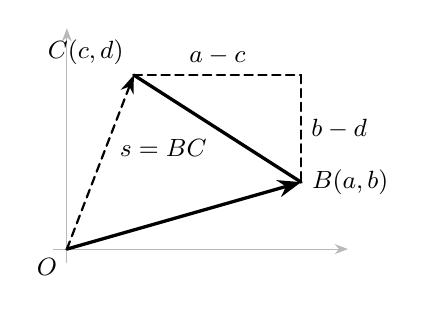
\begin{tikzpicture}[panel,scale=.85]
\draw[faint,->] (-.2,0)--(4.2,0);\draw[faint,->] (0,-.2)--(0,3.3);
\draw[uvec] (0,0)--(3.5,1) node[right] {$B(a,b)$};
\draw[vvec] (0,0)--(1,2.6) node[above left] {$C(c,d)$};
\draw[focus] (1,2.6)--(3.5,1) node[midway,below left] {$s=BC$};
\draw[high] (1,2.6)--(3.5,2.6) node[midway,above] {$a-c$};
\draw[high] (3.5,2.6)--(3.5,1) node[midway,right] {$b-d$};
\node[below left] at (0,0) {$O$};\end{tikzpicture}}
\pausepredict{Why can we equate the two expressions despite the different views?}{Both calculate the squared length of the same segment $BC$. A rigid change of view preserves that length.}
\newpage
\subsection*{Equate, subtract, and divide}
\teach{Remove the common squared lengths}{Abbreviate $S=a^2+b^2+c^2+d^2$ and $G=\norm{\vect u}\norm{\vect v}\cos\theta$. Then
\[
\begin{aligned}
S-2(ac+bd)&=S-2G,\\
[S-2(ac+bd)]-S&=[S-2G]-S,\\
-2(ac+bd)&=-2G,\\
\frac{-2(ac+bd)}{-2}&=\frac{-2G}{-2},\\
ac+bd&=G=\vect u\cdot\vect v.
\end{aligned}
\]
Subtracting the same $S$ preserves equality; dividing by the nonzero scalar $-2$ preserves it too.}{\textbf{Algebraic comparison}\par\medskip
\fbox{\parbox{.88\linewidth}{\centering One segment $BC$\\[5pt]Two formulas for $s^2$\\[5pt]$\downarrow$ subtract $S$\\[5pt]$\downarrow$ divide by $-2$\\[5pt]One coordinate formula}}}
\keyeq{\vect u\cdot\vect v=ac+bd.}
If $\vect u=\vect0$, then $a=b=0$ and $ac+bd=0$. The same argument applies if $\vect v=\vect0$, so the theorem holds for every pair.
\teach{Read the sign as alignment}{For nonzero vectors, $pq>0$. The sign of the dot product equals that of $\cos\theta$:
\[
\begin{array}{c|c}
\theta<90^\circ&\vect u\cdot\vect v>0\\
\theta=90^\circ&\vect u\cdot\vect v=0\\
\theta>90^\circ&\vect u\cdot\vect v<0
\end{array}
\]
For non-collinear pairs these are the acute, perpendicular, and obtuse cases. At the collinear endpoints, $\theta=0$ gives positive and $\theta=\pi$ negative alignment.}{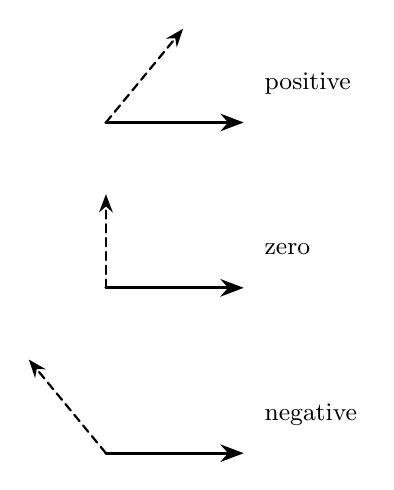
\begin{tikzpicture}[panel,scale=.7]
\foreach \xx/\lab/\yy in {1.4/positive/0,0/zero/-3,-1.4/negative/-6}{
\begin{scope}[yshift=\yy cm]
\draw[uvec] (0,0)--(2.5,0);\draw[vvec] (0,0)--(\xx,1.7);
\node[right] at (2.7,.7) {\lab};\end{scope}}
\end{tikzpicture}}
\newpage
\subsection*{Useful identities follow from the proved formula}
\tagword{Length and symmetry}
\[
\vect u\cdot\vect u=a\cdot a+b\cdot b=a^2+b^2=\norm{\vect u}^2,
\qquad
\vect v\cdot\vect u=ca+db=ac+bd=\vect u\cdot\vect v.
\]
These identities use ordinary scalar multiplication of coordinates.

\tagword{Distributivity} Let $\vect w=(e,f)$. Distribute in coordinates and regroup:
\[
\begin{aligned}
(\vect u+\vect w)\cdot\vect v
&=(a+e)c+(b+f)d\\
&=ac+ec+bd+fd\\
&=(ac+bd)+(ec+fd)\\
&=\vect u\cdot\vect v+\vect w\cdot\vect v.
\end{aligned}
\]
Similarly, for any scalar $t$,
\[
(t\vect u)\cdot\vect v=(ta)c+(tb)d=t(ac+bd)=t(\vect u\cdot\vect v).
\]
Symmetry gives linearity in the other input as well. This is bilinearity.

\textbf{Algebraic grouping schematic (not a geometric area diagram).}
\[
\underbrace{ac+bd}_{\vect u\cdot\vect v}
\quad+\quad
\underbrace{ec+fd}_{\vect w\cdot\vect v}.
\]
The terms are grouped by which vector supplied the first coordinate factor.
\pausepredict{Can the dot product alone tell clockwise from counterclockwise?}{No. Reflecting a pair reverses its orientation while keeping its lengths and unoriented angle. The cosine, and hence the dot product, stays the same. We need a perpendicular measurement with a sign convention.}


\newpage
\section{Base times height: the parallelogram area}
We first find ordinary, nonnegative area $A$. Orientation will come later.
\teach{Start with the two adjacent sides}{Place $\vect u$ and $\vect v$ tail-to-tail. The segment $OB$ will be the base, of length $p=\norm{\vect u}$. The sloping side $OC$ has length $q=\norm{\vect v}$.

This sequence keeps the same $O,B,C$ throughout.}{\parapanel{0}}
\teach{Complete by vector addition}{Translate $\vect v$ to start at $B$, and translate $\vect u$ to start at $C$. Their tips coincide at $W$, because
\[
\overrightarrow{OW}=\vect u+\vect v.
\]
Thus $OBWC$ is a parallelogram. Opposite sides are parallel and equal.}{\parapanel{1}}
\teach{Measure perpendicular height}{Drop $CH\perp OB$. The distance between the parallel lines $OB$ and $CW$ is
\[
h=CH=q\sin\theta.
\]
The dashed height is shorter than the sloping side unless the angle is right. Area depends on this perpendicular distance.}{\parapanel{2}}
\newpage
\subsection*{Why base times height gives the area}
\teach{Cut off one right triangle}{Use the pictured configuration $O=(0,0)$, $B=(4,0)$, $C=(1,2)$, $W=(5,2)$ and $H=(1,0)$. Here $0<OH<OB$, so the cut $CH$ lies inside the parallelogram.

Cut along $CH$. The triangle $OHC$, marked $T$, separates from the remaining trapezoid $HBWC$.}{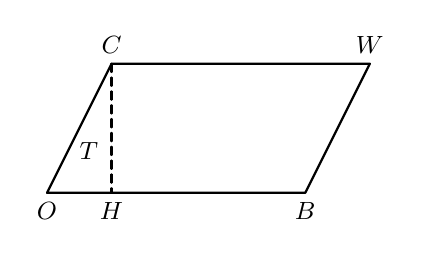
\begin{tikzpicture}[panel,scale=.82]
\path[shade] (0,0)--(4,0)--(5,2)--(1,2)--cycle;
\path[fill=\ifGTenHighlights gray!20\else none\fi] (0,0)--(1,0)--(1,2)--cycle;
\draw[thick] (0,0)--(4,0)--(5,2)--(1,2)--cycle;
\draw[high] (1,2)--(1,0);
\node at (.65,.65) {$T$};\node[below] at (0,0) {$O$};\node[below] at (1,0) {$H$};
\node[below] at (4,0) {$B$};\node[above] at (1,2) {$C$};\node[above] at (5,2) {$W$};
\end{tikzpicture}}
\teach{Translate the matching piece}{Move $T$ by $\vect u=(4,0)$. Then $O\mapsto B$, $H\mapsto K=(5,0)$, and $C\mapsto W$. The translated triangle is $BKW$, also marked $T$.

Translation preserves area. The two pieces fill rectangle $HKWC$ with width $HK=OB=p$ and height $h$. Hence $A=ph$.}{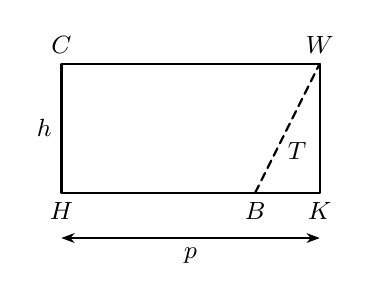
\begin{tikzpicture}[panel,scale=.82]
\path[shade] (1,0)--(4,0)--(5,2)--(1,2)--cycle;
\path[fill=\ifGTenHighlights gray!20\else none\fi] (4,0)--(5,0)--(5,2)--cycle;
\draw[thick] (1,0) rectangle (5,2);\draw[high] (4,0)--(5,2);
\node at (4.65,.65) {$T$};\node[below] at (1,0) {$H$};\node[below] at (4,0) {$B$};\node[below] at (5,0) {$K$};
\node[above] at (1,2) {$C$};\node[above] at (5,2) {$W$};
\draw[<->] (1,-.7)--(5,-.7) node[midway,below] {$p$};\node[left] at (1,1) {$h$};
\end{tikzpicture}}
\textbf{Why the conclusion extends.} A left-slanting parallelogram can be reflected to use the same dissection. If the horizontal offset exceeds a base length, cut the figure into finitely many horizontal strips so each strip's offset is smaller than $p$. Each strip has base length $p$ and the demonstrated area $p$ times its height. Adding the strip areas gives $p$ times the total height. Zero height gives zero area.
\[
A=ph=p(q\sin\theta)=\norm{\vect u}\norm{\vect v}\sin\theta\qquad(0\le\theta\le\pi).
\]
If either vector is zero, the figure collapses and $A=0$. For a directed angle $\varphi$, the unsigned formula uses $|\sin\varphi|$.
\newpage
\section{Deriving the determinant formula from the area identity}
\tagword{Goal} Eliminate the angle from the area formula. Here $A$ remains unsigned.
\teach{Square the geometric formula}{Start with $A=pq\sin\theta$. Squaring gives
\[
A^2=p^2q^2\sin^2\theta.
\]
The square records the size, but cannot retain an orientation sign. That sign has not yet been assigned.}{\parapanel{2}}
\teach{Replace sine squared}{Pythagoras gave $\sin^2\theta=1-\cos^2\theta$. Therefore
\[
\begin{aligned}
A^2&=p^2q^2(1-\cos^2\theta)\\
&=p^2q^2-p^2q^2\cos^2\theta.
\end{aligned}
\]
This uses the complementary along-base and perpendicular components of the same $\vect v$.}{\trianglepanel{3}}
\teach{Recognize the squared dot product}{Since $pq\cos\theta=\vect u\cdot\vect v$,
\[
\begin{aligned}
p^2q^2\cos^2\theta&=(pq\cos\theta)^2,\\
A^2&=p^2q^2-(\vect u\cdot\vect v)^2.
\end{aligned}
\]
Now substitute the proved coordinate formulas:
\[
A^2=(a^2+b^2)(c^2+d^2)-(ac+bd)^2.
\]}{\textbf{Algebraic substitutions}\par\medskip
$\begin{aligned}
p^2&\longmapsto a^2+b^2\\[5pt]
q^2&\longmapsto c^2+d^2\\[5pt]
pq\cos\theta&\longmapsto ac+bd
\end{aligned}$
\par\medskip Each replacement is an identity already proved.}
\newpage
\subsection*{Expand, cancel, factor, and take the nonnegative root}
\teach{Keep all expansion terms visible}{Distribute both products:
\[
\begin{aligned}
(a^2+b^2)(c^2+d^2)
&=a^2c^2+a^2d^2\\&\quad+b^2c^2+b^2d^2,\\
(ac+bd)^2&=a^2c^2+abcd\\&\quad+abcd+b^2d^2.
\end{aligned}
\]
Subtract the entire second row. Both $abcd$ terms receive a minus sign.}{\textbf{Algebraic term map}\par\smallskip
\renewcommand{\arraystretch}{1.5}
\begin{tabular}{c|c|c}
product&subtract square&result\\\hline
$a^2c^2$&$-a^2c^2$&$0$\\
$b^2d^2$&$-b^2d^2$&$0$\\
$a^2d^2$&---&$a^2d^2$\\
$b^2c^2$&---&$b^2c^2$\\
---&$-abcd-abcd$&$-2abcd$
\end{tabular}
\par\smallskip These fourth-degree terms are algebraic quantities, not literal areas in the original plane.}
\teach{Cancel matching terms and factor}{The two matching pairs cancel. The remaining terms form a perfect square:
\[
\begin{aligned}
A^2&=a^2d^2-2abcd+b^2c^2\\
&=(ad)^2-2(ad)(bc)+(bc)^2\\
&=(ad-bc)(ad-bc)\\
&=(ad-bc)^2.
\end{aligned}
\]
Use $r^2-2rt+t^2=(r-t)^2$, with $r=ad$ and $t=bc$.}{\textbf{Factoring schematic}\par\medskip
$\begin{array}{c|cc}
\times&ad&-bc\\\hline
ad&(ad)^2&-abcd\\
-bc&-abcd&(bc)^2
\end{array}$
\par\medskip Reading the four cells backwards reconstructs the factors.}
\teach{Select the nonnegative square root}{Physical area satisfies $A\ge0$. Thus
\[
A=\sqrt{A^2}=\sqrt{(ad-bc)^2}=|ad-bc|.
\]
Both $t$ and $-t$ square to $t^2$; its nonnegative root is $|t|$. For instance $\sqrt{(-6)^2}=6$, not $-6$.}{\fbox{\parbox{.88\linewidth}{\centering Unsigned area\\$A=|ad-bc|\ge0$\\[8pt]Signed expression\\$ad-bc$ may be\\positive, zero, or negative.}}}
\tagword{Definition} With vectors as columns,
\[
D(\vect u,\vect v):=\det\begin{pmatrix}a&c\\b&d\end{pmatrix}:=ad-bc,
\qquad A=|D(\vect u,\vect v)|.
\]
The expression is $ad-bc$, not $ac-bd$. Transposing gives the same determinant, provided entries are placed consistently. If a vector is zero, both sides of the area identity are zero too.
\newpage
\section{Signed area, orientation, and the meaning of subtraction}
\tagword{Orientation convention} The ordered basis $(\vect e_1,\vect e_2)$ is positive. A non-collinear ordered pair is positive when the smaller directed turn from $\vect u$ to $\vect v$ is counterclockwise, and negative when it is clockwise. We justify this sign by signed height, independently of the squared-area identity.
\teach{Normalize the base direction}{For $\vect u=(a,b)\ne\vect0$, put $p=\sqrt{a^2+b^2}>0$. Divide by $p$:
\[
\vect e_{\parallel}=\frac{\vect u}{p}=\left(\frac a p,\frac b p\right).
\]
The new arrow points along $\vect u$ but has length $1$.}{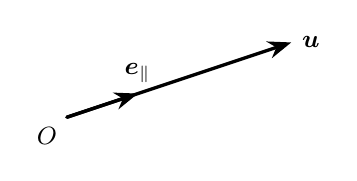
\begin{tikzpicture}[panel,scale=.95]
\draw[uvec] (0,0)--(3,1) node[right] {$\vect u$};
\draw[focus,->] (0,0)--(.94868,.31623) node[above] {$\vect e_{\parallel}$};
\node[below left] at (0,0) {$O$};\end{tikzpicture}}
\teach{Turn the unit direction counterclockwise}{A $90^\circ$ counterclockwise rotation sends $(r,s)$ to $(-s,r)$. Hence
\[
\vect e_{\perp}=\left(-\frac b p,\frac a p\right).
\]
Check both requirements:
\[
\begin{aligned}
\vect e_{\parallel}\cdot\vect e_{\perp}
&=-ab/p^2+ab/p^2=0,\\
\norm{\vect e_{\perp}}^2&=(b^2+a^2)/p^2=1.
\end{aligned}
\]
This chooses a particular perpendicular side: the positive side of the ordered base.}{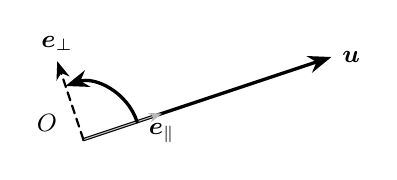
\begin{tikzpicture}[panel,scale=1.05]
\draw[uvec] (0,0)--(3,1) node[right] {$\vect u$};
\draw[faint,->] (0,0)--(.94868,.31623) node[below] {$\vect e_{\parallel}$};
\draw[high,->] (0,0)--(-.31623,.94868) node[above] {$\vect e_{\perp}$};
\draw[focus,->] (.65,.2167) arc[start angle=18.435,end angle=108.435,radius=.685];
\node[left] at (-.2,.2) {$O$};\end{tikzpicture}}
\newpage
\subsection*{Project onto the positive perpendicular}
\teach{Read and calculate signed height}{Let $k=\vect v\cdot\vect e_{\perp}$. This projection is positive on the $\vect e_{\perp}$ side and negative on the opposite side:
\[
\begin{aligned}
k&=(c,d)\cdot\left(-\frac b p,\frac a p\right)\\
&=-\frac{bc}{p}+\frac{ad}{p}=\frac{ad-bc}{p}.
\end{aligned}
\]
The physical height is $h=|k|$. The vector projection is $k\vect e_{\perp}$, whereas $k$ itself is a scalar.}{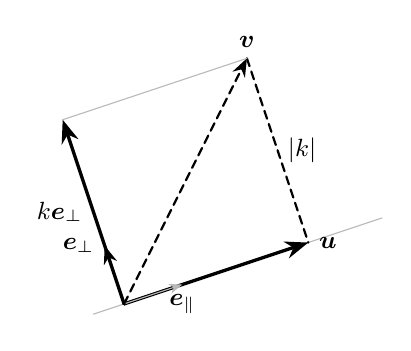
\begin{tikzpicture}[panel,scale=.78]
\draw[faint] (-.5,-.1667)--(4.2,1.4);
\draw[uvec] (0,0)--(3,1) node[right] {$\vect u$};
\draw[vvec] (0,0)--(2,4) node[above] {$\vect v$};
\draw[faint,->] (0,0)--(.94868,.31623) node[below] {$\vect e_{\parallel}$};
\draw[high,->] (0,0)--(-.31623,.94868) node[left] {$\vect e_{\perp}$};
\draw[high] (2,4)--(3,1) node[midway,right] {$|k|$};
\draw[faint] (2,4)--(-1,3);
\draw[focus,->] (0,0)--(-1,3) node[midway,left] {$k\vect e_{\perp}$};
\end{tikzpicture}}
\teach{Multiply by the positive base length}{Multiply by $p>0$:
\[
pk=p\frac{ad-bc}{p}=ad-bc=D(\vect u,\vect v).
\]
Thus $D$ is base length times \emph{signed} height; $A=p|k|=|D|$ is unsigned.

If $\varphi\in(-\pi,\pi]$ is the directed angle from $\vect u$ to $\vect v$, then
\[
k=q\sin\varphi,\qquad D=pq\sin\varphi.
\]
Unlike $\theta\in[0,\pi]$, $\varphi$ keeps the turning direction.}{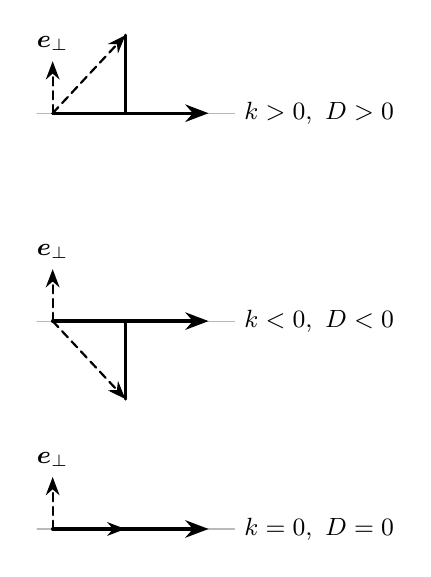
\begin{tikzpicture}[panel,scale=.66]
\foreach \yy/\hh/\lab in {0/1.5/{$k>0,\ D>0$},-4/-1.5/{$k<0,\ D<0$},-8/0/{$k=0,\ D=0$}}{
\begin{scope}[yshift=\yy cm]
\draw[faint] (-.3,0)--(3.5,0);\draw[uvec] (0,0)--(3,0);
\draw[vvec] (0,0)--(1.4,\hh);\draw[high,->] (0,0)--(0,1) node[above] {$\vect e_{\perp}$};
\draw[focus] (1.4,0)--(1.4,\hh);
\node[right] at (3.5,0) {\lab};\end{scope}}
\end{tikzpicture}}
\pausepredict{Could $A^2=D^2$ alone have told us which side is positive?}{No. The counterclockwise choice of $\vect e_{\perp}$ supplies the convention; the projection calculation proves that $ad-bc$ obeys it.}
\newpage
\subsection*{Order changes sign; dependence collapses area}
\teach{Swap the ordered arrows on the same figure}{The parallelogram is unchanged. Only the order of the two starting arrows is reversed:
\[
\begin{aligned}
D(\vect v,\vect u)&=cb-da\\
&=bc-ad=-(ad-bc)\\
&=-D(\vect u,\vect v).
\end{aligned}
\]
A counterclockwise turn becomes clockwise. The area stays the same because $|-D|=|D|$.}{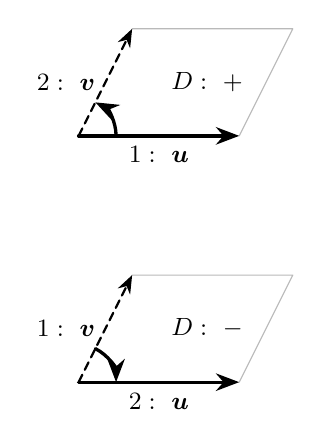
\begin{tikzpicture}[panel,scale=.68]
\foreach \shift/\first/\second/\sgn in {0/{1:\ \vect u}/{2:\ \vect v}/+,-4.6/{2:\ \vect u}/{1:\ \vect v}/-}{
\begin{scope}[yshift=\shift cm]
\path[shade] (0,0)--(3,0)--(4,2)--(1,2)--cycle;
\draw[faint] (3,0)--(4,2)--(1,2);
\draw[uvec] (0,0)--(3,0) node[midway,below] {$\first$};
\draw[vvec] (0,0)--(1,2) node[midway,left] {$\second$};
\node at (2.4,1) {$D:\ \sgn$};\end{scope}}
\draw[focus,->] (.7,0) arc[start angle=0,end angle=63.435,radius=.7];
\draw[focus,<-] (.7,-4.6) arc[start angle=0,end angle=63.435,radius=.7];
\end{tikzpicture}}
\teach{Check parallel and perpendicular pairs}{If $\vect v=t\vect u$, then $c=ta$, $d=tb$, and
\[
D(\vect u,t\vect u)=a(tb)-b(ta)=0.
\]
Conversely, for $\vect u\ne\vect0$, $D=pk=0$ forces $k=0$. Thus $\vect v$ is parallel to $\vect u$.

For a nonzero perpendicular pair, $\vect u\cdot\vect v=0$, but $|D|=pq>0$. If either vector is zero, both products are zero.}{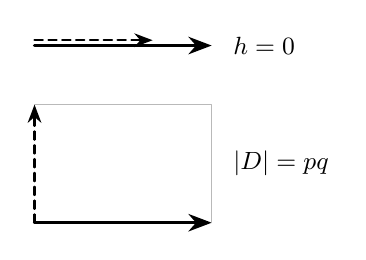
\begin{tikzpicture}[panel,scale=.75]
\draw[uvec] (0,0)--(3,0);\draw[vvec] (0,.09)--(2,.09);
\node[right] at (3.2,0) {$h=0$};
\draw[uvec] (0,-3)--(3,-3);\draw[vvec] (0,-3)--(0,-1);
\draw[faint] (3,-3)--(3,-1)--(0,-1);
\node[right] at (3.2,-2) {$|D|=pq$};\end{tikzpicture}}


\newpage
\section{Three worked examples}
\subsection*{Example 1: angle, dot product, and area}
Take $\vect u=(3,1)$ and $\vect v=(2,4)$. These panels keep the original coordinate axes and the same unit scale.
\teach{Place the coordinates and calculate lengths}{The tips are $B=(3,1)$ and $C=(2,4)$:
\[
\begin{aligned}
\vect u\cdot\vect v&=3(2)+1(4)=6+4=10,\\
p&=\sqrt{3^2+1^2}=\sqrt{10},\\
q&=\sqrt{2^2+4^2}=\sqrt{20}.
\end{aligned}
\]
The positive dot product predicts an acute included angle.}{\examplepanel{0}}
\teach{Find the projection and included angle}{The scalar projection along $\vect u$ is
\[
x=\frac{\vect u\cdot\vect v}{p}=\frac{10}{\sqrt{10}}=\sqrt{10}=p.
\]
So the perpendicular foot is exactly $B$. From the geometric definition,
\[
\begin{aligned}
\cos\theta&=\frac{10}{\sqrt{10}\sqrt{20}}\\
&=\frac{10}{\sqrt{200}}=\frac1{\sqrt2},\\
\theta&=45^\circ.
\end{aligned}
\]
Indeed $C-B=(-1,3)$ is perpendicular to $\vect u$, since $3(-1)+1(3)=0$.}{\examplepanel{1}}
\newpage
\subsection*{Example 1 continued: turn the same picture into an area}
\teach{Complete the parallelogram and find height}{The fourth vertex is $W=B+C=(5,5)$. The perpendicular height is $BC$:
\[
\begin{aligned}
h&=q\sin45^\circ=\frac{\sqrt{20}}{\sqrt2}=\sqrt{10},\\
A&=ph=\sqrt{10}\sqrt{10}=10.
\end{aligned}
\]
Equivalently,
\[
A=\sqrt{200}\frac1{\sqrt2}=10\sqrt2\frac1{\sqrt2}=10.
\]
The dashed $BC$ is a height, not the sloping side $OC$.}{\examplepanel{2}}
\teach{Check the determinant and orientation}{Calculate in the original coordinates:
\[
\begin{aligned}
D(\vect u,\vect v)&=3(4)-1(2)\\
&=12-2=10,\\
A&=|10|=10.
\end{aligned}
\]
The determinant agrees with the geometric area. It is positive because the turn $OB\to OC$ is counterclockwise.

The signed height is $k=D/p=\sqrt{10}>0$, consistent with $\vect v$ lying on the counterclockwise side of $\vect u$.}{\examplepanel{3}}
\newpage
\subsection*{Example 2: parallel vectors}
\teach{See the collapsed parallelogram}{Let $\vect u=(3,1)$ and $\vect v=(6,2)=2\vect u$. All four vertices $O,B,C,W=(9,3)$ lie on one line:
\[
\begin{aligned}
D(\vect u,\vect v)&=3(2)-1(6)\\
&=6-6=0,\\
A&=|0|=0.
\end{aligned}
\]
The vectors point in the same direction, so $\theta=0$. The height is $q\sin0=0$; the projected tip $H$ coincides with $C$.}{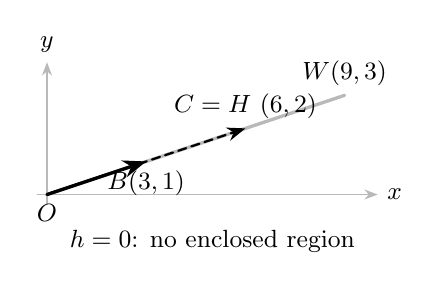
\begin{tikzpicture}[panel,scale=.42]
\draw[faint,->] (-.3,0)--(10,0) node[right] {$x$};\draw[faint,->] (0,-.3)--(0,4) node[above] {$y$};
\draw[faint,very thick] (0,0)--(9,3);
\draw[vvec] (0,0)--(6,2);\draw[uvec] (0,0)--(3,1);
\node[below] at (0,0) {$O$};\node[below] at (3,1) {$B(3,1)$};
\node[above] at (6,2) {$C=H\ (6,2)$};\node[above] at (9,3) {$W(9,3)$};
\node at (5,-1.4) {$h=0$: no enclosed region};\end{tikzpicture}}
\subsection*{Example 3: an obtuse clockwise pair}
\teach{Separate the two negative signs}{Let $\vect u=(2,0)$ and $\vect v=(-1,-3)$:
\[
\begin{aligned}
\vect u\cdot\vect v&=2(-1)+0(-3)=-2<0,\\
D(\vect u,\vect v)&=2(-3)-0(-1)=-6<0,\\
A&=|-6|=6.
\end{aligned}
\]
The along-base projection is $x=-1$: the unoriented angle is obtuse. The signed height is $k=-3$: the directed turn is clockwise. The physical height is $3$.

These signs describe different facts. Reflecting $C$ above the horizontal axis reverses $D$ while keeping the dot product negative.}{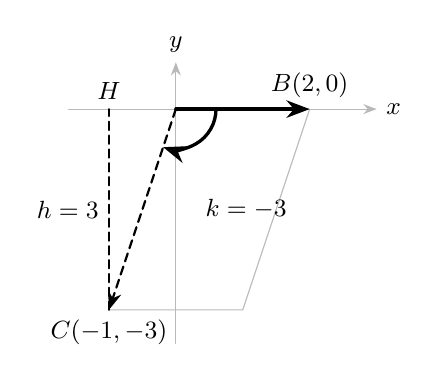
\begin{tikzpicture}[panel,scale=.85]
\draw[faint,->] (-1.6,0)--(3,0) node[right] {$x$};\draw[faint,->] (0,-3.5)--(0,.7) node[above] {$y$};
\path[shade] (0,0)--(2,0)--(1,-3)--(-1,-3)--cycle;
\draw[faint] (2,0)--(1,-3)--(-1,-3);
\draw[uvec] (0,0)--(2,0) node[above] {$B(2,0)$};
\draw[vvec] (0,0)--(-1,-3) node[below] {$C(-1,-3)$};
\draw[high] (-1,-3)--(-1,0) node[midway,left] {$h=3$};
\node[above] at (-1,0) {$H$};
\draw[focus,->] (.6,0) arc[start angle=0,end angle=-108.435,radius=.6];
\node[right] at (.3,-1.5) {$k=-3$};\end{tikzpicture}}
\newpage
\section{An optional next step: the wedge product}
\textbf{Question.} Can we keep the oriented area element itself, rather than just its number? The wedge product gives such an object, called a \emph{bivector}.

\tagword{Definition (exterior algebra in the plane)} For $V=\R^2$,
\[
\Lambda(V)=\Lambda^0(V)\oplus\Lambda^1(V)\oplus\Lambda^2(V),
\]
where $\Lambda^0(V)\cong\R$, $\Lambda^1(V)=V$, and $\Lambda^2(V)$ is one-dimensional with basis $\vect e_1\wedge\vect e_2$. The product is bilinear and alternating on vectors:
\[
\begin{aligned}
(\vect x+\vect y)\wedge\vect z&=\vect x\wedge\vect z+\vect y\wedge\vect z,\\
\vect x\wedge(\vect y+\vect z)&=\vect x\wedge\vect y+\vect x\wedge\vect z,\\
(\lambda\vect x)\wedge\vect y&=\lambda(\vect x\wedge\vect y),\\
\vect x\wedge(\lambda\vect y)&=\lambda(\vect x\wedge\vect y),\\
\vect x\wedge\vect x&=0.
\end{aligned}
\]
These are defining properties, not deductions from the determinant formula.

\textbf{Step 1. Derive reversal of order.} Alternation applied to $\vect x+\vect y$, followed by bilinearity, gives
\[
\begin{aligned}
0&=(\vect x+\vect y)\wedge(\vect x+\vect y)\\
&=\vect x\wedge\vect x+\vect x\wedge\vect y
+\vect y\wedge\vect x+\vect y\wedge\vect y\\
&=0+\vect x\wedge\vect y+\vect y\wedge\vect x+0.
\end{aligned}
\]
Subtracting $\vect x\wedge\vect y$ gives $\vect y\wedge\vect x=-\vect x\wedge\vect y$.

\textbf{Step 2. Expand before simplifying.} Distribute the left factor, then the right factor, then bring scalars outside:
\[
\begin{aligned}
\vect u\wedge\vect v
&=(a\vect e_1+b\vect e_2)\wedge(c\vect e_1+d\vect e_2)\\
&=(a\vect e_1)\wedge(c\vect e_1+d\vect e_2)
 +(b\vect e_2)\wedge(c\vect e_1+d\vect e_2)\\
&=(a\vect e_1)\wedge(c\vect e_1)+(a\vect e_1)\wedge(d\vect e_2)\\
&\quad+(b\vect e_2)\wedge(c\vect e_1)+(b\vect e_2)\wedge(d\vect e_2)\\
&=ac(\vect e_1\wedge\vect e_1)+ad(\vect e_1\wedge\vect e_2)\\
&\quad+bc(\vect e_2\wedge\vect e_1)+bd(\vect e_2\wedge\vect e_2).
\end{aligned}
\]
Keep all four terms. The next grid explains each basis pair. Coefficient signs remain in the algebra; the grid depicts basis orientations, not scaled component vectors.
\newpage
\subsection*{Four basis pairs, four terms}
\[
\begin{aligned}
\vect u\wedge\vect v
&=ac(\vect e_1\wedge\vect e_1)+ad(\vect e_1\wedge\vect e_2)\\
&\quad+bc(\vect e_2\wedge\vect e_1)+bd(\vect e_2\wedge\vect e_2).
\end{aligned}
\]
\textbf{Basis-orientation schematics.} Numerals mark the \emph{first} and \emph{second} inputs. Coefficients $ac,ad,bc,bd$ are not represented by arrow lengths.
\begin{center}
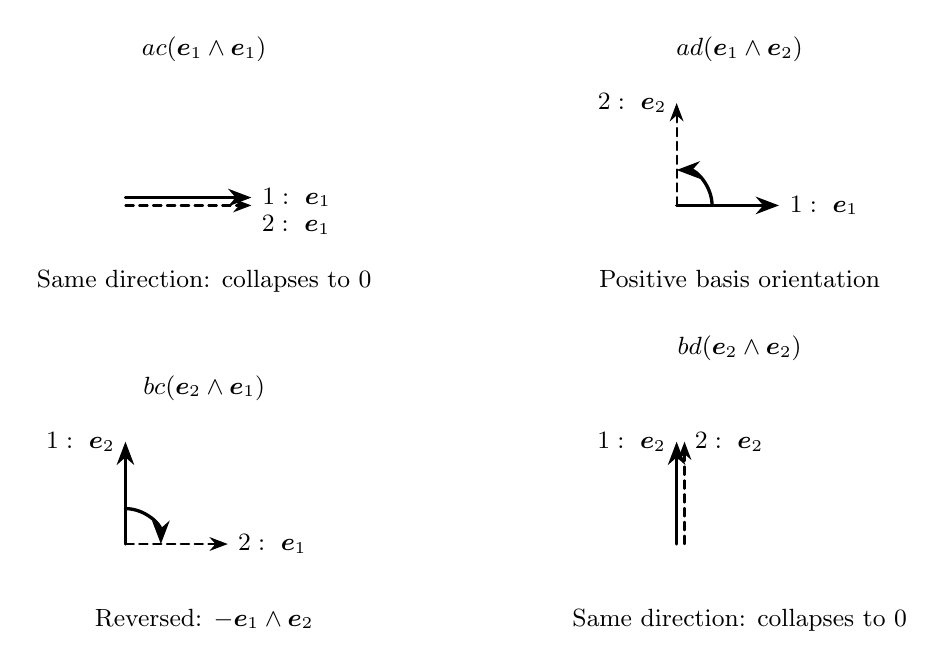
\begin{tikzpicture}[panel,scale=1]
\begin{scope}
\node[above] at (1,1.7) {$ac(\vect e_1\wedge\vect e_1)$};
\draw[uvec] (0,.1)--(1.6,.1) node[right] {$1:\ \vect e_1$};
\draw[vvec] (0,0)--(1.6,0) node[below right] {$2:\ \vect e_1$};
\node[below] at (1,-.7) {Same direction: collapses to $0$};
\end{scope}
\begin{scope}[xshift=7cm]
\node[above] at (.8,1.7) {$ad(\vect e_1\wedge\vect e_2)$};
\path[shade] (0,0) rectangle (1.3,1.3);
\draw[uvec] (0,0)--(1.3,0) node[right] {$1:\ \vect e_1$};
\draw[vvec] (0,0)--(0,1.3) node[left] {$2:\ \vect e_2$};
\draw[focus,->] (.45,0) arc[start angle=0,end angle=90,radius=.45];
\node[below] at (.8,-.7) {Positive basis orientation};
\end{scope}
\begin{scope}[yshift=-4.3cm]
\node[above] at (1,1.7) {$bc(\vect e_2\wedge\vect e_1)$};
\path[shade] (0,0) rectangle (1.3,1.3);
\draw[uvec] (0,0)--(0,1.3) node[left] {$1:\ \vect e_2$};
\draw[vvec] (0,0)--(1.3,0) node[right] {$2:\ \vect e_1$};
\draw[focus,->] (0,.45) arc[start angle=90,end angle=0,radius=.45];
\node[below] at (1,-.7) {Reversed: $-\vect e_1\wedge\vect e_2$};
\end{scope}
\begin{scope}[xshift=7cm,yshift=-4.3cm]
\node[above] at (.8,2.2) {$bd(\vect e_2\wedge\vect e_2)$};
\draw[uvec] (0,0)--(0,1.3) node[left] {$1:\ \vect e_2$};
\draw[vvec] (.1,0)--(.1,1.3) node[right] {$2:\ \vect e_2$};
\node[below] at (.8,-.7) {Same direction: collapses to $0$};
\end{scope}
\end{tikzpicture}
\end{center}
Parallel arrows are offset slightly for visibility; they represent a collapsed area, not a thin strip.

\textbf{Step 3. Substitute the basis relations and collect.}
\[
\begin{aligned}
\vect u\wedge\vect v
&=ac(0)+ad(\vect e_1\wedge\vect e_2)
+bc(-\vect e_1\wedge\vect e_2)+bd(0)\\
&=0+ad(\vect e_1\wedge\vect e_2)-bc(\vect e_1\wedge\vect e_2)+0\\
&=(ad-bc)(\vect e_1\wedge\vect e_2).
\end{aligned}
\]
\keyeq{\vect u\wedge\vect v=\det\begin{pmatrix}a&c\\b&d\end{pmatrix}(\vect e_1\wedge\vect e_2).}
The bivector is the whole expression. The scalar $ad-bc$ is its coefficient \emph{relative to the chosen oriented basis element} $\vect e_1\wedge\vect e_2$. Swapping vectors changes its sign. Parallel or zero vectors give the zero bivector.
\newpage
\subsection*{Optional perspective beyond the plane}
In $\R^3$ and higher, wedge products still encode oriented area, but $\Lambda^2(V)$ generally has several independent basis bivectors. Thus the wedge product is not merely another notation for a single plane determinant. The exterior product extends associatively to higher grades. Homogeneous elements satisfy graded commutativity
\[
\alpha\wedge\beta=(-1)^{k\ell}\beta\wedge\alpha,
\qquad\alpha\in\Lambda^k(V),\quad\beta\in\Lambda^\ell(V).
\]
\section{Synthesis: two complementary geometric measurements}
\begin{center}
\renewcommand{\arraystretch}{1.28}
\begin{tabular}{@{}p{.23\linewidth}p{.32\linewidth}p{.36\linewidth}@{}}
\toprule
\textbf{Question}&\textbf{Dot product}&\textbf{Determinant}\\\midrule
Geometric meaning&Alignment / signed projection&Signed area / orientation\\
Angle dependence&$\norm{\vect u}\norm{\vect v}\cos\theta$&$\norm{\vect u}\norm{\vect v}\sin\varphi$\\
Coordinates&$ac+bd$&$ad-bc$\\
Zero for nonzero pair&Perpendicular&Parallel\\
On swapping vectors&Unchanged&Sign reversed\\
\bottomrule
\end{tabular}
\end{center}
Here $\theta\in[0,\pi]$ is an unoriented angle, whereas $\varphi$ is directed from $\vect u$ to $\vect v$. A nonzero vector pair can never be simultaneously perpendicular and parallel.

\textbf{Central idea.} The dot product measures how much one vector lies \emph{along} another; the determinant measures its signed \emph{perpendicular} component, multiplied by the base length. The wedge product keeps the corresponding oriented area element as an algebraic object.

\newpage
\section*{Check your understanding}
\begin{enumerate}
\item For $\vect u=(1,2)$ and $\vect v=(3,-1)$, compute the dot product and unsigned area. Determine whether the unoriented angle is acute or obtuse, and whether the orientation is positive or negative.
\item Can two nonzero vectors have dot product zero and determinant zero simultaneously? Justify using the geometric meanings, not only coordinates.
\item If $\vect v$ is replaced by $3\vect v$, how do dot product, determinant, and unsigned area change? Repeat for $-\vect v$.
\item Starting from $A^2=\norm{\vect u}^2\norm{\vect v}^2-(\vect u\cdot\vect v)^2$, explain precisely why squaring does not determine orientation.
\item Reproduce the law of cosines for an obtuse angle by writing the signed projection $x<0$. Identify the point where Pythagoras enters.
\item Expand $(2\vect e_1-\vect e_2)\wedge(\vect e_1+3\vect e_2)$ term by term, then check the coefficient against a $2\times2$ determinant.
\end{enumerate}
\end{document}
